\section{Software and Device drivers}
The Wupper tools communicate with the Wupper core through the Wupper device driver. Buffers in the host PC memory are used for bidirectional data transfers, this is done by a part of the driver called CMEM. This will reserve a chunk of contiguous memory in the host. For the specific case of the example application, the allocated memory will be logically subdivided in two buffers (buffer 1 and buffer 2 in Figure~\ref{fig:wupperpackage}). One buffer is used to store data coming from the FPGA (write buffer, buffer 1), the other to store the ones going to the FPGA (read buffer, buffer 2). The idea behind the logical split of the memory in buffers is that those buffers can be used to copy data from the write to read, and perform checks. The driver is developed for Scientific Linux CERN 6 but has been tested and used also under Ubuntu kernel version 3.13.0-44a. Building and loading/unloading the driver is explained in \ref{sec:buildloadDrivers}.

In this chapter we assume that the card is loaded with the latest firmware, it has been placed in a Gen3 PCIe slot and the PC is running Linux. Optionally a Vivado hardware server can be connected to view the Debug probes of the ILA cores, as specified in the constraints file. \cite{programming}\

\subsection{Building / Loading the drivers}
\label{sec:buildloadDrivers}
The Drivers for Wupper consist of two parts. The first part is the cmem driver, this driver allocates a contiguous block of RAM in the PC memory which can be used for the DMA transfers.

The second part is the Wupper driver which allows access to the DMA descriptors and the registermap.
\begin{lstlisting}[language=BASH, frame=single, caption=Building and Loading the driver]
#build the driver
cd trunk/hostSoftware/driver
./makedrivers
# load the driver
sudo scripts/drivers_wupper start
# see status of the driver
sudo scripts/drivers_wupper status
# unload the driver
sudo scripts/drivers_wupper stop
\end{lstlisting}
\subsection{Driver functionality}
Before any DMA actions can be performed, one or more memory buffers have to be allocated. The driver in conjunction with the wupper tools take this into account. 

The application has to do two important tasks for a DMA action to occur.
\begin{itemize}
	\item Allocate a buffer using the CMEM driver
	\item Create and enable the DMA descriptor.
\end{itemize}

If the buffer is for instance allocated at address 0x00000004d5c00000, initialize bits 64:0 of the descriptor with 0x00000004d5c00000, and end address (bit 127:64) 0x00000004d5c00000 plus the write size. If a \underline{DMA Write} is to be performed, initialize bits 10:0 of descriptor 0a with 0x40 (for 256 bytes per TLP, depending on the PC chipset) and bit 11 with '0' for write, then enable the corresponding descriptor enable bit at address 0x400. The TLP size of 0x40 (32 bit words) is limited by the maximum TLP that the PC can handle, in most cases this is 256 bytes, the Engine can handle bigger TLP's up to 4096 bytes.
\begin{lstlisting}[language=BASH, frame=single, caption=Create a Write descriptor]
#write descriptor 0
#BAR0 offset:  Contents:
0x0000         0x00000004d5c00000
0x0008         0x00000004d5c00400
#Set the length to 0x40 / Write
0x0010         0x040
#enable descriptor 0 to start the DMA Write
0x0400         1
\end{lstlisting}
If a \underline{DMA Read} of 1024 bytes (0x100 DWords) from PC memory is to be performed at address 0x00000004d5d00000, initialize bits 64:0 of the descriptor with 0x00000004d5d00000, and bits [127:64] with 0x00000004d5d00400. Initialize bits 10:0 of descriptor 0 with 0x100 and bit 11 with '1' for read, then enable the corresponding descriptor enable bit at address 0x400. The TLP size of 0x100 is limited by the maximum TLP size of the Xilinx core, set to 1024 bytes, 0x100 words.
\begin{lstlisting}[language=BASH, frame=single, caption=Create a Read descriptor]
#write descriptor 1
#BAR0 offset:  Contents:
0x0020         0x00000004d5d00000
0x0028         0x00000004d5d00400
#Set the length to 0x100 / Read
0x0030         0x0900
#enable descriptor 1 to start the DMA Read
0x0400         2
\end{lstlisting}


\subsection{Reading and Writing Registers and setting up DMA}

The PCIe Engine has a register map with 128 bit address space per register, however registers can be read and written in words of 32, 64, 96 or 128 bits at a time. The addresses of the register have an offset with respect to a Base Address Register (BAR) that can be readout running: The PCIe Engine has 3 different BAR spaces all with their own memory map. 

BAR0 is the memory area which contains registers that are related to DMA operations. The most important registers are the descriptors.

BAR1 is the memory area which contains registers that are related to Interrupt vectors.

BAR2 is the user memory area, it contains some example registers which can be implemented per the requirements for the user / application.

\subsection{Wupper tools}
The Wupper tools are a collection of tools which can be used to debug and control the Wupper core. These tools are command line programs and can only run if the device driver is loaded. A detailed list and explanation of each tool is given in the next paragraphs. Some tools are specific to the example VHDL application, some other tools are more generic and can directly be used to control the Wupper DMA core, the Wupper-dma-transfer and Wupper-chaintest had been added as features for the OpenCores' benchmark example application. As mentioned before, the purpose of those applications is to check the health of the Wupper core. 

The Wupper tools can be found in the directory hostSoftware/wupper\_tools.

The Wupper tools collection comes with a readme~\cite{wupperreadme}, this explains how to compile and run the tools. Most of the tools have an -h option to provide helpful information. 

\begin{lstlisting}[language=BASH, frame=single, caption=Building Wupper Tools]
cd trunk/hostSoftware/wupper_tools
mkdir build
cd build
cmake ..
make
\end{lstlisting}
The build directory should now contain the following tools. All the tools come with a "-h" option to show a help message.

\begin{center}
	\begin{tabular}{ | l || p{10cm} |}
		\hline
		Tool & Description                       \\ \hline
		
		Wupper-info
		&  Prints information of the device. For instance device ID, PLL lock status of the internal clock and FW version.
		\\ \hline
		
		Wupper-reset
		&  Resets parts of the example application core. These functions are also implemented in the Wupper-dma-transfer tool.
		\\ \hline
		
		
		Wupper-config
		& Shows the PCIe configuration registers and allows to set, store and load configuration. An example is configuring the LED's on the VC-709 board by writing a hexadecimal value to the register.
		\\ \hline
		Wupper-irq-test
		&  Tool to test interrupt routines
		\\ \hline
		
		Wupper-dma-test
		& This tool transfers every second 1024 Byte of data and dumps it to the screen.
		\\ \hline
		
		Wupper-throughput
		&  The tool measures the throughput of the Wupper core. The method of computing the throughput is wrong, this is discussed in the section 3.4.2.
		\\ \hline
		
		
		Wupper-dump-blocks
		&  This tools dumps a block of 1 KB. The iteration is set standard on 100. This can be changed by adding a number after the "-n".
		\\ \hline
		
	\end{tabular}
\end{center}

\newpage
\subsubsection{Operating Wupper-dma-transfer}

Wupper-dma-transfer sends data to the target PC via Wupper also known as half loop test. This tool operates the benchmark application and has multiple options. A list of such options is summarized in Listing~\ref{lst:dmatoollist}.

\begin{lstlisting}[language=BASH, frame=single, label={lst:dmatoollist}, caption=Output of Wupper-dma-transfer -h]
daqmustud@gimone:$ ./wupper-dma-transfer -h

Usage: wupper-dma-transfer [OPTIONS]


This application has a sequence: 
1 -Start with dma reset(-d)
2 -Flush the FIFO's(-f)
3 -Then reset the application (-r)


Options:
-l             Load pre-programmed seed.
-q             Load and generate an unique seed.
-g             Generate data from PCIe to PC.
-b             Generate data from PC to PCIe.
-s             Show application register.
-r             Reset the application.
-f             Flush the FIFO's.
-d             Disable and reset the DMA controller.
-h             Display help.


\end{lstlisting}


Before using the write function, make sure that the application is ready by resetting all the values, as shown in Listing~\ref{lst:dmatoolreset}.

\begin{lstlisting}[language=BASH, frame=single, label={lst:dmatoolreset},  caption=Reset Wupper before a DMA Write action]
daqmustud@gimone:$ ./wupper-dma-transfer -d
Resetting the DMA controller...DONE! 
daqmustud@gimone:$ ./wupper-dma-transfer -f
Flushing the FIFO's...DONE! 
daqmustud@gimone:$ ./wupper-dma-transfer -r
resetting application...DONE! 
\end{lstlisting}


\newpage

\newpage

\noindent
Before writing data into the PC, the data generator needs a seed to initialize the generator. There are two options available: load a unique seed or load a pre-programmed seed. The pre-programmed seed is always 256 bits, the unique seed value can be variable. The -s option displays the status of the register including the seed value. For a unique seed, replace the -l with -q, as shown in Listing~\ref{lst:dmatoolseed}.

\begin{lstlisting}[language=BASH, frame=single, label={lst:dmatoolseed}, caption=Loading a pre-programmed seed in to the data generator.]
daqmustud@gimone:$ ./wupper-dma-transfer -l
Writing seed to application register...DONE! 
daqmustud@gimone:$ ./wupper-dma-transfer -s

Status application registers
----------------------------
LFSR_SEED_0A:        DEADBEEFABCD0123 
LFSR_SEED_0B:        87613472FEDCABCD 
LFSR_SEED_1A:        DEADFACEABCD0123 
LFSR_SEED_1B:        12313472FEDCFFFF 
APP_MUX:             0 
LFSR_LOAD_SEED:      0
\end{lstlisting}


The -g option performs a DMA write to the PC memory. The data generator starts to fill the down FIFO and from the PC side, a DMA read action is performed. The size of the transfer is set to 1 MB by default, but the size is configurable. When the PC receives 1 MB of data, the transfer stops. It is possible that there is still some data left in the down FIFO, resetting the FIFO's can be done by the -f option, as shown in Listing~\ref{lst:dmatoolwrite}.

\begin{lstlisting}[language=BASH, frame=single, label={lst:dmatoolwrite}, caption=Start generating data to the target.]
daqmustud@gimone:$ ./wupper-dma-transfer -g
Starting DMA write
done DMA write 
Buffer 1 addresses:
0: EED9733362A50D71 
...
...
...
\end{lstlisting}

\newpage

In a similar way a DMA read action from the FPGA can be performed by using the -b option. The output of the up FIFO is fed to a multiplier. The output of the multiplier is fed to the down FIFO with a destination to the PC memory as shown in Listing~\ref{lst:dmatoolback}.

\begin{lstlisting}[language=BASH, frame=single, label={lst:dmatoolback}, caption= Performing a DMA read and DMA write]
daqmustud@gimone:$ ./wupper-dma-transfer -b
Reading data from buffer 1...
DONE!
Buffer 2 addresses:
0: 24BBEC63B53F3BCC 
...
...
...
\end{lstlisting}

\subsubsection{Operating Wupper-chaintest}
The Wupper-chaintest tool does in one shot a complete DMA Read and Write transfer. It checks if the multiplied data is done correctly. This is done by multiplying the data in buffer 2 and compare the output of the multiplier in buffer 1 (shown earlier in Figure~\ref{fig:wupperpackage}). The tool returns the number of errors out of 65536 loops as shown in Listing~\ref{lst:chaintest}.
\begin{lstlisting}[language=BASH, frame=single, label={lst:chaintest}, caption=Output of Wupper-chaintest]
daqmustud@gimone:$ ./wupper-chaintest      
Reading data from buffer 1...
DONE!
Buffer 2 addresses:
0: 49A5A89745420D34 
...
...
... 
9: 5D37679AE79FA7C2 
0 errors out of 65536
\end{lstlisting}

\newpage


\subsection {Wupper GUI}

The Wupper Gui is a dedicated application for the example vhdl application, as described in \ref{sec:ExampleApp}. The concept of the Wupper GUI is based on the Wupper tools and has the same construction (see Figure~\ref{fig:softwaretree}). The GUI is developed with Qt version 5.5 (C++ based)~\cite{qt} and gives the user a visual feedback of the Wupper's status/health. The GUI can only run if the device driver is loaded.

\begin{figure}[h]
	\centering
	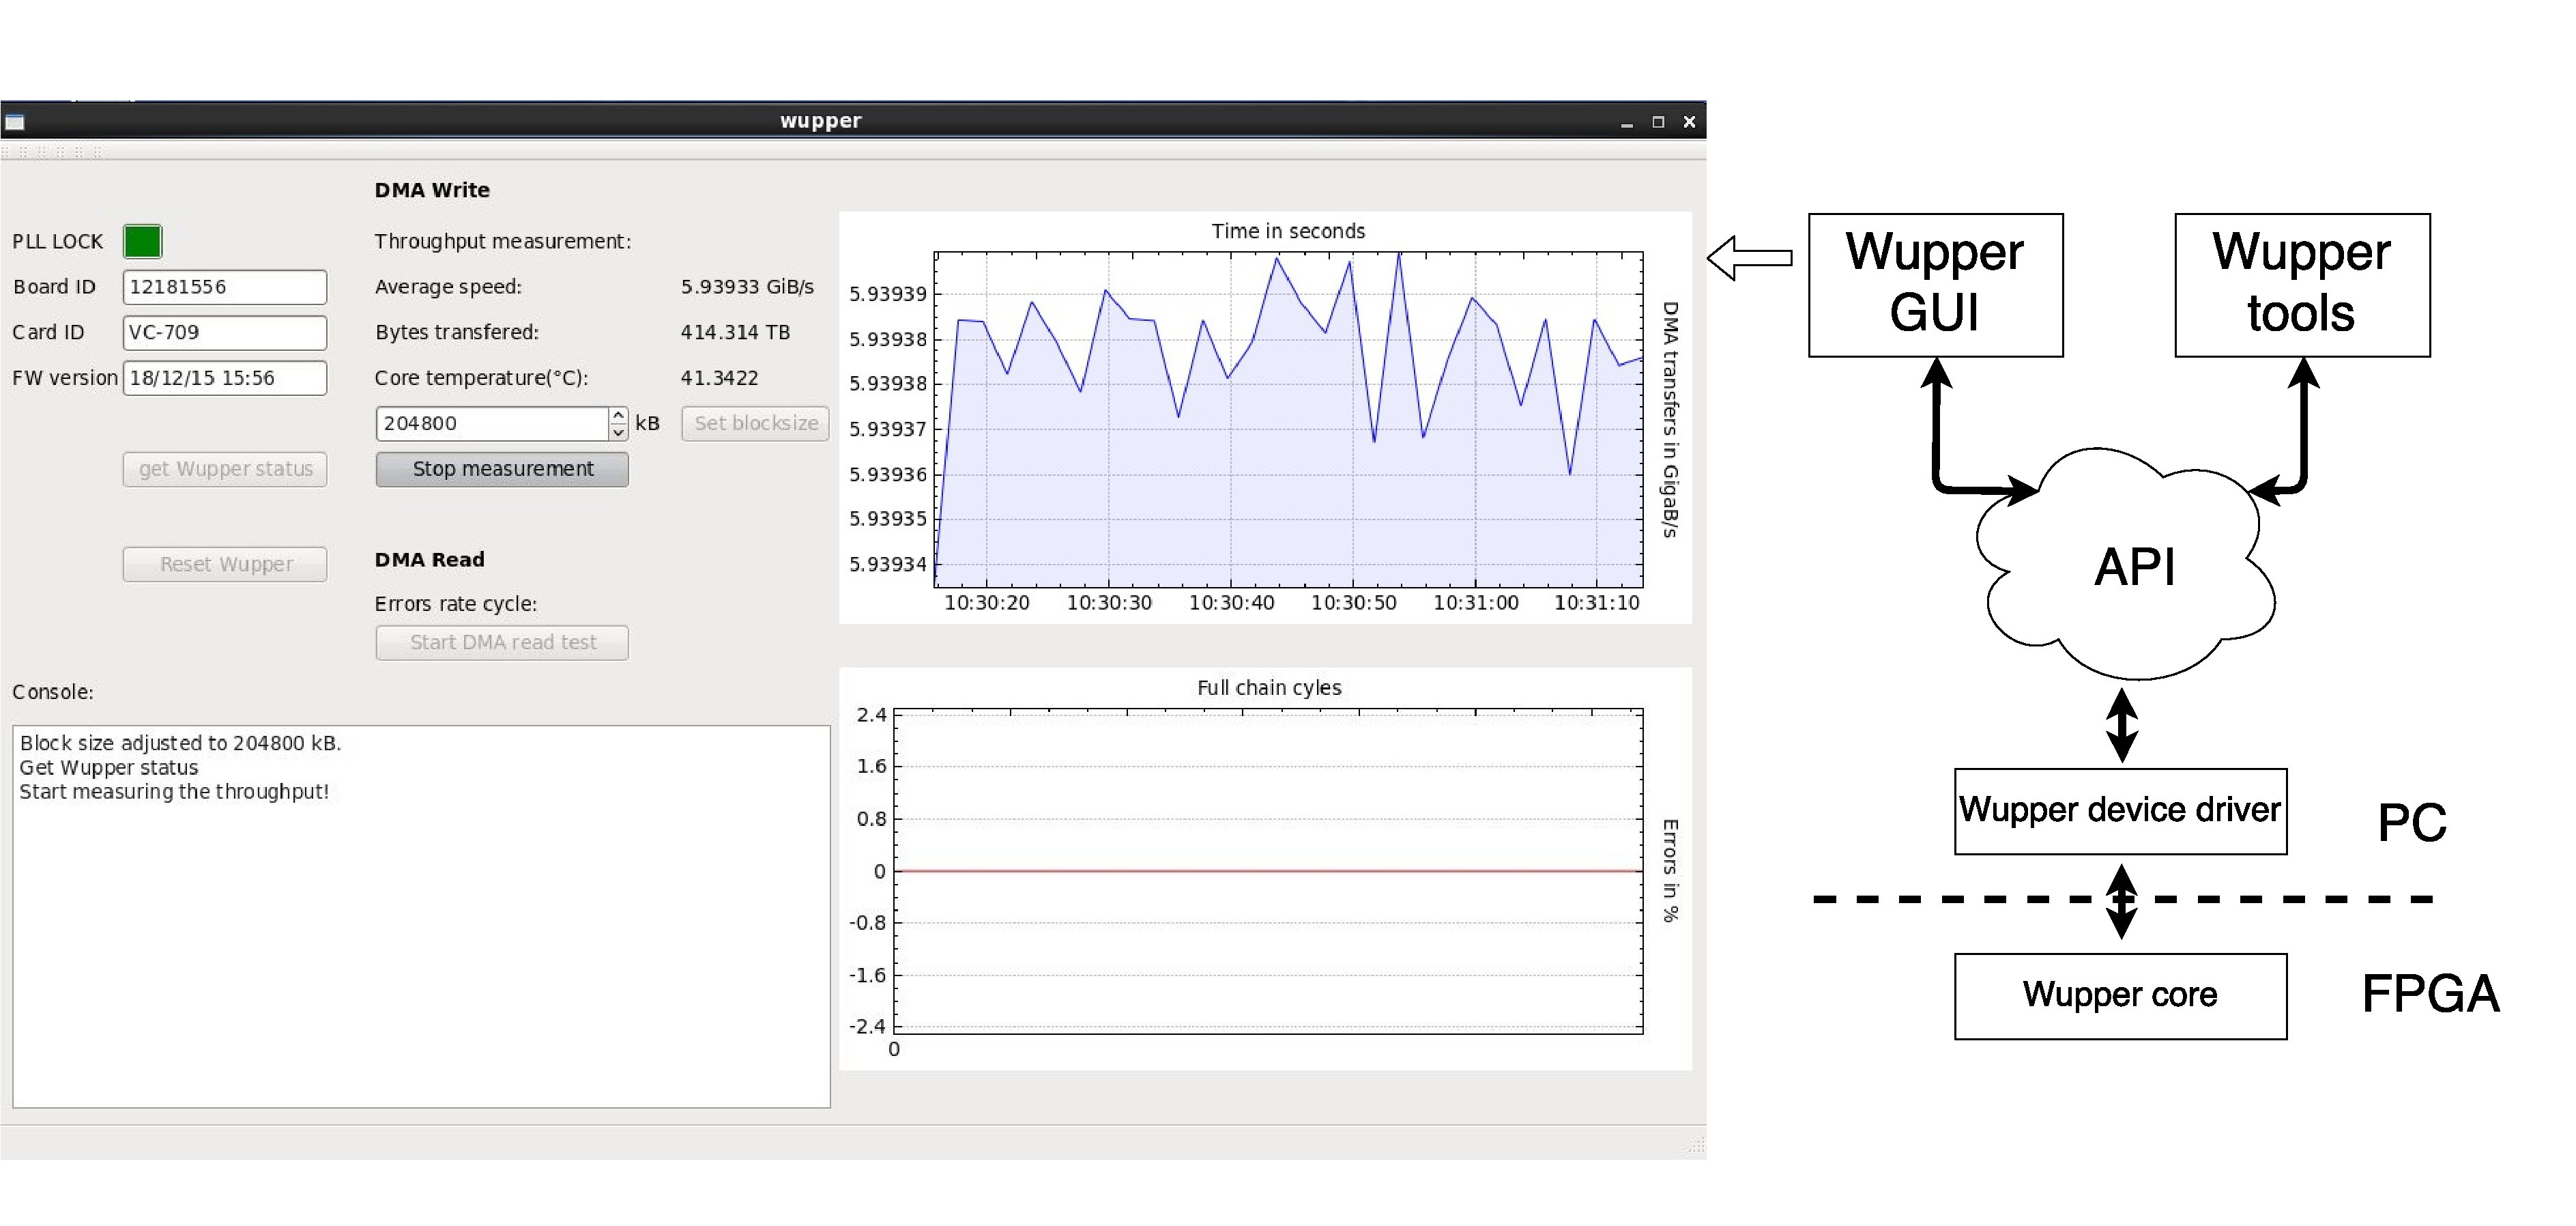
\includegraphics[width = 0.7 \textwidth]{figures/tree.pdf}	
	\caption{High and low level software overview block diagram.}
	\label{fig:softwaretree}
\end{figure}

\subsubsection {Functional blocks and threaded programming}


Multi-threading is used so functional blocks can run at the same time as the GUI. If multi-threading is not used, the GUI interface gets stuck. A thread starts a new process next to the main process. If another processor core is available, the thread will run on a separated core. By communicating via slots to the main process, the data is secured.
There are two threads but only one of the threads can be used at the same time. The reason is that both threads use the same DMA ID, this will cause an error.
The threads communicate with the Application Program Interface (API) to control and fetch the output of the logic. The output data communicate safely via a signal to the slots. Figure~\ref{fig:guithreads} shows an overview of the threaded programs in the Wupper GUI.

\begin{figure}[h]
	\centering
	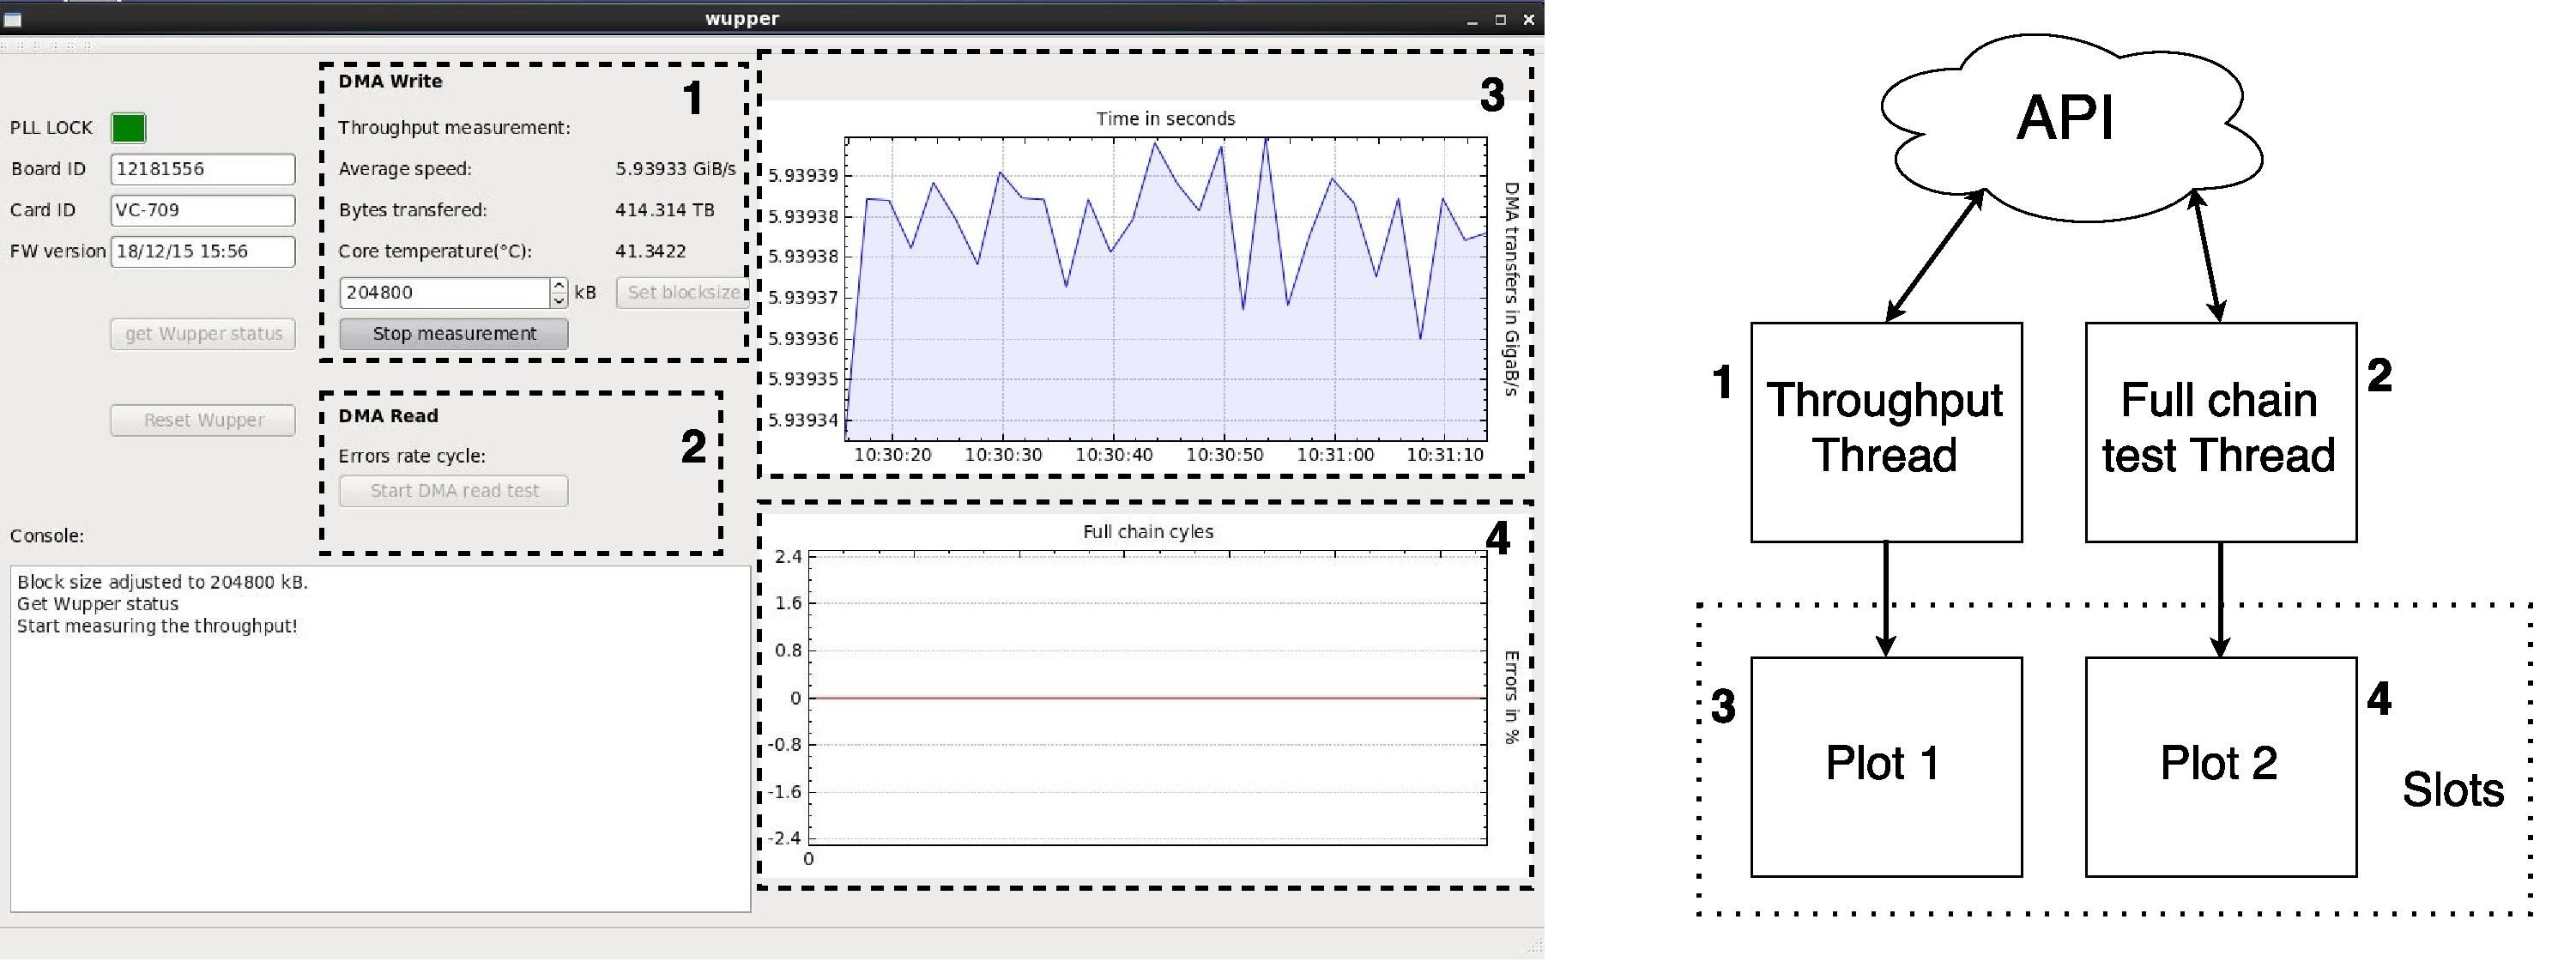
\includegraphics[width = 0.9 \textwidth]{figures/wupper_gui_threads_overview.pdf}	
	\caption{Threaded programs in the Wupper GUI}
	\label{fig:guithreads}
\end{figure}

\newpage
\subsubsection {GUI operation}

The GUI is separated in four regions (see Figure~\ref{fig:wuppergui}): status, control, measurement and an info region.
The status region fetches the information about various parts of the FPGA on the VC-709 via the Wupper core, and about the core itself. When the user clicks on the "get Wupper status" button, it shows the internal PLL lock status, Board ID, Card ID and the firmware version.

The control region controls the logic inside Wupper through the API. The "Reset Wupper" button resets the application logic by resetting the DMA, flushing the FIFO's and reset the application values. 

In the DMA Write section, the user can perform a DMA Write measurement. The user can configure the blocksize. The blocksize has effect on the speed, this is discussed in Appendix ~\ref{sec:blocksize}. The measurement output is shown in the measurement region. The method of computing the throughput is different than the method of the Wupper-throughput tool. The fault is the wrong order of operations by misplacing brackets. The wrong method is $A/B*C= D$ instead of $A/(B*C)= D$.

In a similar way, the user can perform a DMA Read test and the output is shown in the plot in the measurement region.
The info/console output region gives the user feedback of the application and the GUI.

\begin{figure}[h]
	\centering
	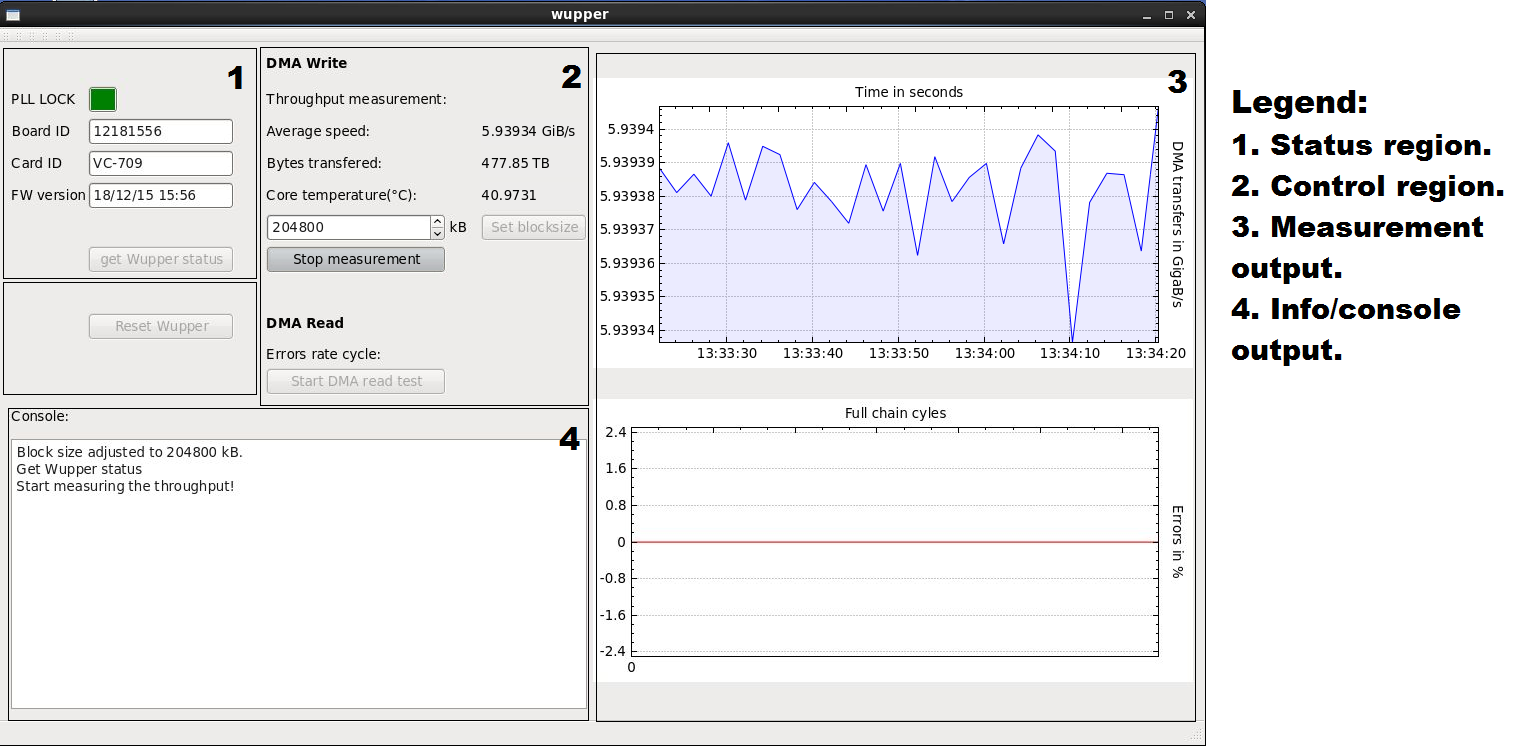
\includegraphics[width = 1 \textwidth]{figures/gui_printscreen_tb.PNG}	
	\caption{Screenshot of the example application GUI}
	\label{fig:wuppergui}
\end{figure}






\newpage